\documentclass[crop,tikz]{standalone}

\usetikzlibrary{positioning}
\usepackage[utf8]{inputenc}

% 'crop' is the default for v1.0, before it was 'preview'
\usetikzlibrary{decorations.markings}

\newcommand{\sphere}[2]{
	\begin{scope}[shift={#2}]
	  	\shade[ball color = gray!10, opacity = 1] (0,0) circle (#1);
  		\draw (0,0) circle (#1);
	\end{scope}
} %\sphere{radius}{(xshift,yshift)} - note: centred on 0,0

\newcommand{\vertex}[2]{
	\sphere{0.25}{#1}
	\node at #1 {#2};
} %\vertex{position}{caption}

\newcommand{\clearcube}[2]{
	\begin{scope}[shift={#2}]
		\draw[thick, dashed] (-#1,-#1,#1) -- (-#1,-#1,-#1) -- (#1,-#1,-#1);
		\draw[thick, dashed] (-#1,-#1,-#1) -- (-#1,#1,-#1);
		\draw[thick] (-#1,-#1,#1) -- (#1,-#1,#1) -- (#1,-#1,-#1) -- (#1,#1,-#1) -- (#1,#1,#1) -- (#1,-#1,#1);
		\draw[thick] (#1,#1,#1) -- (-#1,#1,#1) -- (-#1,-#1,#1);
		\draw[thick] (-#1,#1,#1) -- (-#1,#1,-#1) -- (#1,#1,-#1);
	\end{scope}
} %\cube{side length/2}{(xshift,yshift,zshift)} - note: centred on 0,0,0

\newcommand{\fillcube}[4]{
	\begin{scope}[shift={#2}]
		\draw[gray, thick, dashed] (-#1,-#1,-#1) -- (-#1,-#1,#1) -- (-#1,#1,#1) -- (-#1,#1,-#1) -- cycle;
		\filldraw[#3, opacity=#4] (-#1,-#1,-#1) -- (-#1,-#1,#1) -- (-#1,#1,#1) -- (-#1,#1,-#1) -- cycle;
		\draw[gray, thick, dashed] (#1,-#1,-#1) -- (#1,-#1,#1) -- (#1,#1,#1) -- (#1,#1,-#1) -- cycle;
		\filldraw[#3, opacity=#4] (#1,-#1,-#1) -- (#1,-#1,#1) -- (#1,#1,#1) -- (#1,#1,-#1) -- cycle;
		\draw[gray, thick, dashed] (-#1,-#1,#1) -- (-#1,#1,#1) -- (#1,#1,#1) -- (#1,-#1,#1) -- cycle;
		\filldraw[#3, opacity=#4] (-#1,-#1,#1) -- (-#1,#1,#1) -- (#1,#1,#1) -- (#1,-#1,#1) -- cycle;
		\draw[gray, thick, dashed] (-#1,-#1,-#1) -- (-#1,#1,-#1) -- (#1,#1,-#1) -- (#1,-#1,-#1) -- cycle;
		\filldraw[#3, opacity=#4] (-#1,-#1,-#1) -- (-#1,#1,-#1) -- (#1,#1,-#1) -- (#1,-#1,-#1) -- cycle;
		\draw[gray, thick, dashed] (-#1,-#1,-#1) -- (-#1,-#1,#1) -- (#1,-#1,#1) -- (#1,-#1,-#1) -- cycle;
		\filldraw[#3, opacity=#4] (-#1,-#1,-#1) -- (-#1,-#1,#1) -- (#1,-#1,#1) -- (#1,-#1,-#1) -- cycle;
		\draw[gray, thick, dashed] (-#1,#1,-#1) -- (-#1,#1,#1) -- (#1,#1,#1) -- (#1,#1,-#1) -- cycle;
		\filldraw[#3, opacity=#4] (-#1,#1,-#1) -- (-#1,#1,#1) -- (#1,#1,#1) -- (#1,#1,-#1) -- cycle;
	\end{scope}
} %\fillcube{side length/2}{(xshift,yshift,zshift)}{col options}{opacity} - note: centred on 0,0,0

\begin{document}

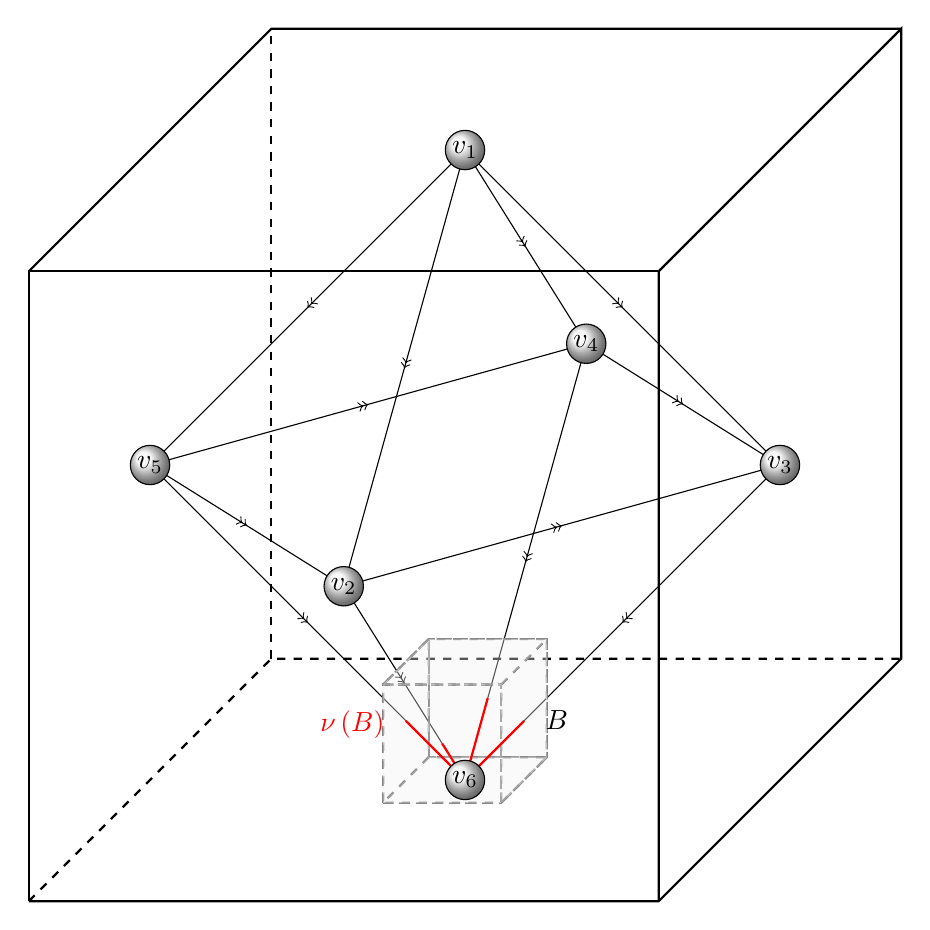
\begin{tikzpicture}
%	%reference unit vectors!
%	\draw[->] (0,0,0) -- (0,0,1) node[anchor=south] {$z$};
%	\draw[->] (0,0,0) -- (0,1,0) node[anchor=south] {$y$};
%	\draw[->] (0,0,0) -- (1,0,0) node[anchor=south] {$x$};

	%3D domain is a cube, draw that
	\clearcube{4}{(0,0,0)}

	%instructions from here on are sensitive to the argument in \cube

	%co-ordinates for the vertices
	\coordinate (FF) at (0,0,4); %FF = Front Face
	\coordinate (BkF) at (0,0,-4); %BkF = Back Face
	\coordinate (TF) at (0,4,0); %TF = Top Face
	\coordinate (BtF) at (0,-4,0); %BtF = Bottom Face
	\coordinate (LF) at (-4,0,0); %LF = Left Face
	\coordinate (RF) at (4,0,0); %RF = Right Face

	%draw edges
	\begin{scope}[decoration={markings, mark=at position 0.5 with {\arrow{>>}}}]
		\draw[postaction={decorate}] (TF) -- (FF);
		\draw[postaction={decorate}] (TF) -- (RF);
		\draw[postaction={decorate}] (TF) -- (BkF);
		\draw[postaction={decorate}] (TF) -- (LF);
		\draw[postaction={decorate}] (FF) -- (BtF);
		\draw[postaction={decorate}] (RF) -- (BtF);
		\draw[postaction={decorate}] (BkF) -- (BtF);
		\draw[postaction={decorate}] (LF) -- (BtF);
		\draw[postaction={decorate}] (LF) -- (BkF);
		\draw[postaction={decorate}] (LF) -- (FF);
		\draw[postaction={decorate}] (BkF) -- (RF);
		\draw[postaction={decorate}] (FF) -- (RF);
	\end{scope}

	%draw the set B
	\fillcube{0.75}{(0,-3.25,0)}{black!5!white}{0.2}
	\node[anchor=north west] at (0.9,-3,0) {$B$};
	%draw red lines to indicate the parts of $B$ that $\nu$ cares about
	\draw[thick, red] (BtF) -- (-0.75,-3.25,0);
	\draw[thick, red] (BtF) -- (0.75,-3.25,0);
	\draw[thick, red] (BtF) -- (0,-3.25,-0.75);
	\draw[thick, red] (BtF) -- (0,-3.25,0.75);
	\node[red, anchor=north east] at (-0.9,-3,0) {$\nu\left(B\right)$};
	
	%draw vertices
	\vertex{(TF)}{$v_1$};	\vertex{(FF)}{$v_2$};	\vertex{(RF)}{$v_3$}; 
	\vertex{(BkF)}{$v_4$};	\vertex{(LF)}{$v_5$};	\vertex{(BtF)}{$v_6$};
	
\end{tikzpicture}

\end{document}